%!TEX root = ../../tcc.tex

\newpage
\section{Tabelas Hash Distribuídas e o Kademlia}

As \glsentrylongpl{dht} surgiram quando buscas em \glspl{p2p} não eram eficientes, fosse
pelos problemas da supercentralização dos sistemas, ou pela falta dela, de modo a se
criar uma maneira híbrida de buscar e localizar recursos nessas redes.

Existem duas formas de se encontrar recursos: busca e endereçamento. A primeira se
baseia no casamento de palavras-chave com as descrições dos recursos, sendo mais
amigável para o usuário, pois não necessita de mecanismos complexos de identificação.
Porém, é menos eficiente, já que necessita da conferência dos conteúdos dos recursos
para saber se são os mesmos. As \glspl*{p2p} descentralizadas utilizavam esta abordagem.

Quando uma rede tem estrutura descentralizada, ocorre o fenômeno chamado de inundação
de mensagens, no qual estas são repassadas entre \glspl*{peer} intermediários até o
\gls*{peer} de destino. Esse repasse excessivo acarreta \gls{overhead} nos \glspl*{peer}
intermediários, além de gerar mensagens falso-negativas.

A segunda forma de se encontrar recursos utiliza endereços que possam identificá-los de
forma única. Dessa maneira, um recurso é exclusivamente identificável, sendo possível
encontrá-lo eficientemente. Contudo, é necessário algum procedimento para se obter seu
nome único, além de uma estrutura organizada por endereços. Historicamente, as
\glspl*{p2p} de estrutura centralizada se baseiam neste método.

Anteriormente ao BitTorrent, nas \glspl*{p2p} de estrutura centralizada, o servidor
central tentava conhecer a situação de cada um dos \glspl*{peer} da rede, enviando
mensagens diretamente a eles. Gerenciar muitos \glspl*{peer} ao mesmo tempo
sobrecarregava o \emph{hardware} do servidor, às vezes forçando o seu desligamento.

Essas formas de organizar esses recursos através da rede utilizam as conexões entre os
diversos \glspl*{peer}, formando redes superpostas (\emph{overlay networks}), que são
redes virtuais que figuram sobre as tradicionais redes IP. Assim, as \glspl*{p2p}
necessitam de funcionalidades eficientes para que um \gls*{peer} possa entrar e sair do
\emph{overlay}, assim como armazenar recursos e encontrá-los (usando endereçamento). Tal
eficiência é conseguida através de \glspl{dht}, onde todas essas funcionalidades
dependem da troca eficiente de mensagens entre \glspl*{peer}.

\begin{figure}[H]
    \centering
    \fbox{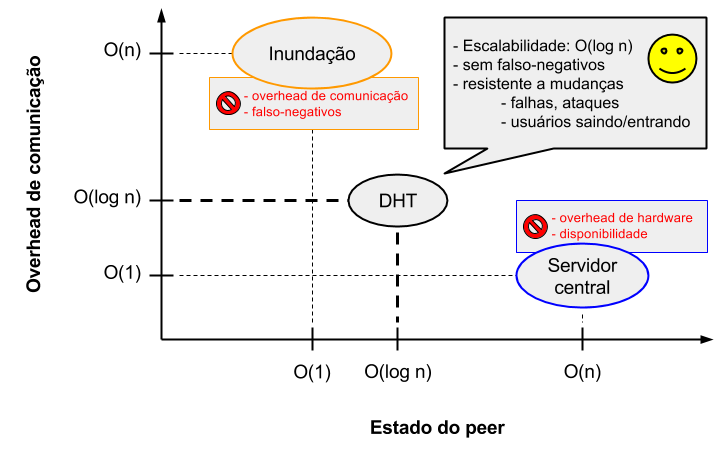
\includegraphics[width=0.85\textwidth]{graph-dht.png}}
    \caption{comparação de overheads de redes centralizadas e descentralizadas, e a
    brecha onde a DHT se encaixa}
    %\label{fig:torrent-universo}
\end{figure}

A \gls*{dht} foi adotada pelos desenvolvedores de programas cliente BitTorrent, mas
sempre como uma funcionalidade particular, sendo utilizada por alguns anos. Tendo
comprovado seu desempenho, foi finalmente adicionada à especificação do BitTorrent no
ano de 2008 \cite{site:bittorrent-dht}.

%!TEX root = ../../tcc.tex

\subsection*{Kademlia}

O Kademlia é uma \gls*{dht}, criada em 2002 \cite{artigo:kademlia}, com o objetivo de
melhorar os métodos de busca atuais (Napster e \gls*{gnutella}), que eram ineficientes.
Assim como os outros algoritmos de \gls*{dht}, ele se baseou na estrutura informalmente
conhecida como \enquote{rede de Plaxton} (\emph{Plaxton mesh}), nome que remete a um
dos seus autores \cite{artigo:dht}. Por ter mostrado bons resultados, foi usado na
implementação da busca de arquivos no programa cliente eMule.

A sua modelagem computacional monta um mapa no formato de \gls*{hashtable} onde IDs de
\glspl*{peer} ou de \glspl*{torrent} são chaves para listas de outros \glspl*{peer}.

%!TEX root = ../../tcc.tex

\subsubsection*{Modelagem e estrutura de dados}

O algoritmo implementa uma rede \emph{overlay} cuja estrutura e comunicação se baseiam
na procura de seus nós. Cada um destes nós é identificado por um identificador único
(ID), que serve tanto para a identificação quanto para a localização de valores na
\gls*{hashtable}.

Essa \gls*{hashtable} é na forma de uma árvore binária, cujas folhas são os nós da rede.
Cada folha tem suas posições estabelecidas pelo menor prefixo comum de seus IDs,
organizando-os de forma que, para um dado nó $x$, a árvore é dividida em várias
subárvores menores que não o contém. Assim, a maior subárvore consiste de metade da
árvore que não contém $x$, a subárvore seguinte é feita da metade da árvore restante
onde $x$ também não está contido, etc. O Kademlia garante ainda que todo nó conhece um
outro que está em cada uma das subárvores, se estas contiverem algum nó.

\begin{figure}[ht!]
    \centering
    \fbox{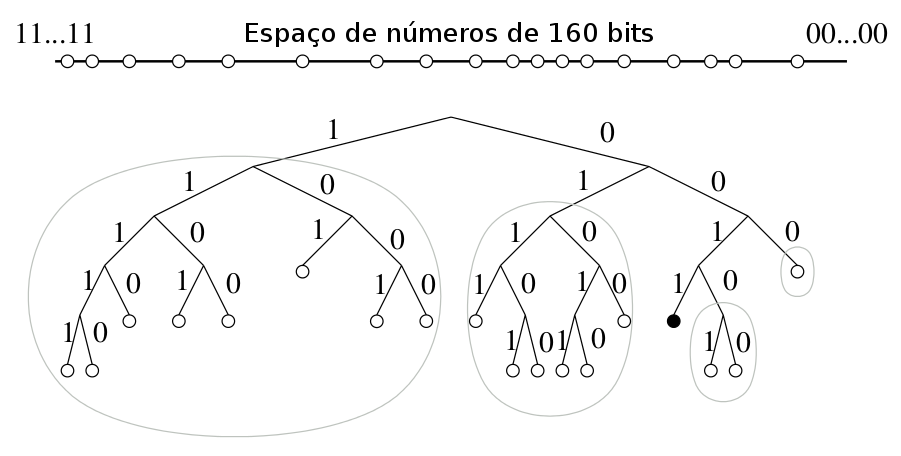
\includegraphics[width=\textwidth]{dht1.png}}
    \caption{Árvore binária do Kademlia. O nó preto é a posição do ID 0011...; os ovais
    cinzas são as subárvores onde o nó preto deve possuir nós conhecidos. Fonte:
    \cite{artigo:kademlia}}
    \label{fig:dht-arvore}
\end{figure}

No Kademlia, objetos e nós possuem IDs únicos de 160 bits: enquanto o primeiro utiliza
o \gls*{hashvalue} de 20 bytes SHA-1 da chave \bverb|info_hash| do \gls*{torrentfile},
o segundo é um valor aleatório escolhido pelo próprio programa.

Durante uma busca por \glspl*{peer} de um \gls*{torrent}, o processo deve conhecer a
chave associado ao objeto, ou seja, o ID, e explora a rede em passos. A cada passo,
encontra nós mais próximos da chave, até chegar ou ao valor buscado ou não nós
existirem mais próximos que o atual. Dessa forma, para uma rede com $n$ nós, o
algoritmo visita apenas $O(\log n)$ nós.

\newpage
\begin{figure}[ht!]
    \centering
    \fbox{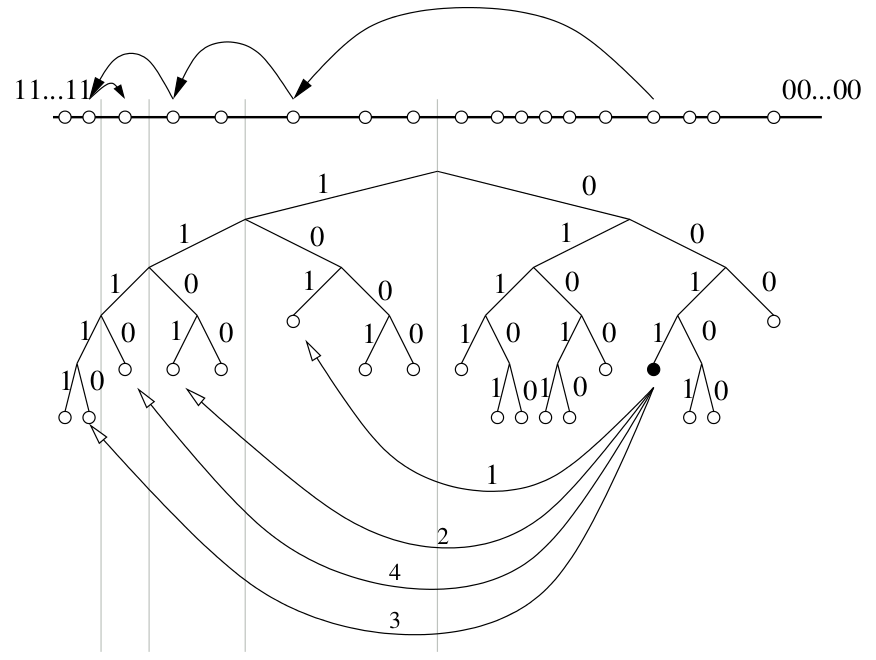
\includegraphics[width=0.8\textwidth]{dht2.png}}
    \caption{Exemplo de uma busca na árvore de nós do Kademlia usando-se um ID. O nó
    preto, de prefixo 0011, encontra o nó de prefixo 1110 através de sucessivas buscas
    (setas numeradas inferiores). As setas superiores mostram a convergência da
    busca durante a execução. Fonte: \cite{artigo:kademlia}}
    \label{fig:dht-arvore-busca}
\end{figure}

Para o conceito de proximidade, as distâncias são calculadas usando-se a função de
distância baseada em \gls{xor} bit a bit

\begin{equation}
    d(x,y) = x \oplus y
\end{equation}

que possui certas propriedades, algumas em comum com a equação de distância euclidiana
usual:

\begin{itemize}
    \item $d(x,x) = 0$
    \item $x \neq y$, $d(x,y) > 0$
    \item simetria: $\forall x,y$, $d(x,y) = d(y,x)$
    \item desigualdade triangular: $d(x,y) + d(y,z) \geq d(x,z)$. \\
        Isto vem do fato de $d(x,z) = d(x,y) \oplus d(y,z)$ e que $\forall a \geq 0,
        \forall b \geq 0 : a + b \geq a \oplus b$
    \item unidirecionalidade: para um dado ponto $x$ e uma distância $\Delta > 0$,
        existe exatamente um ponto $y$ tal que $d(x,y) = \Delta$. Isso garante que todas
        as procuras por uma mesma chave convirjam para um mesmo percurso, independente
        do ponto de partida.
    \item para um dado $x$ no espaço de números, o conjunto de distâncias $\Delta$ entre
        $x$ e os outros números possui distribuição uniforme, ao contrário da distância
        euclidiana \cite{bittorrentcom:dht}
\end{itemize}

No Transmission, o Kademlia é usado a partir de uma biblioteca externa (não mantida
pelos seus desenvolvedores) criada por Juliusz Chroboczek \cite{repo:dht-c}, sendo
adicionada e adaptada para o uso no código do programa. Sua implementação não é na forma
de árvore, mas sim de listas ligadas.

\cfile[label="./third-party/dht/dht.c:129"]{./Codes/chap3/018-dht-structs.c}

%!TEX root = ../../tcc.tex

\subsubsection*{Tabela de roteamento}

Cada nó do \gls*{kademlia} armazena informações sobre outros nós para rotear mensagens
de pesquisa. Para cada bit $i$ dos IDs (cada ID tem 160 bits) é mantido um \gls{kbucket},
que contém os nós cuja distância até ele está entre $2^i$ e $2^{i+1}$. Esses
\glspl*{kbucket} são listas de endereço IP, porta de comunicação \gls*{udp} e ID de
nós, ordenadas pelo horário da última notícia destes. Para distâncias pequenas, essas
listas geralmente serão vazias, enquanto que para distâncias maiores, poderão ser de
tamanho $k$. Este valor, que é o de replicação do sistema, é escolhido de tal forma que
haja grande probabilidade desses $k$ nós não falharem na próxima hora.

Quando um nó \textbf{A} recebe uma mensagem de outro nó \textbf{B}, o \gls*{bucket}
correspondente ao ID do remetente (nó \textbf{B}) é atualizado. Disto, podem ocorrer as
seguintes situações:

\begin{itemize}
    \item \textbf{B} já existe no \gls*{bucket}: passa a ser o primeiro da lista, pois
        existiu mensagem recente;

    \item \textbf{B} não existe no \gls*{bucket}:
        \begin{itemize}
            \item \gls*{bucket} não está cheio: \textbf{B} é adicionado no começo da
                lista;
            \item \gls*{bucket} cheio: é enviado um \emph{ping} para o nó do final da
                lista (nó \textbf{C}), contatado há mais tempo:

                \begin{itemize}
                    \item \textbf{C} não responde ao \emph{ping}: \textbf{C} é retirado
                        da lista e \textbf{B} é inserido no início;
                    \item \textbf{C} responde ao \emph{ping}: \textbf{C} é movido para o
                        início da lista e \textbf{B} é ignorado.
                \end{itemize}
        \end{itemize}
\end{itemize}

Por conta disso, ocorre que nós mais antigos e funcionais são preferidos, pois quanto
mais tempo um nó está conectado, mais provável que ele se mantenha conectado por mais
uma hora \cite{artigo:gnutella-uptime}. Outra vantagem disso é a resistência a alguns
ataques de negação de serviço, pois mesmo que ocorra uma inundação de novos nós, estes
só seriam inseridos nos \glspl*{kbucket} se os antigos fossem excluídos.

%!TEX root = ../../tcc.tex

\subsubsection*{Protocolo}

O protocolo de mensagens \gls*{dht} utiliza o formato KRPC, um mecanismo de \gls{rpc}
que envia dicionários \gls*{bencode} através de \gls*{udp}, uma única vez por chamada
(um pacote para a requisição, outro para a resposta), sem novas tentativas.

Existem três tipos de mensagem: consulta (\emph{query}), resposta (\emph{response}) e
erro (\emph{error}). Para o protocolo \gls*{dht}, são quatro comandos \emph{query}:
\bverb|ping|, \bverb|find_node|, \bverb|get_peers| e \bverb|announce_peer|. Em todos, o
nó sempre enviará seu ID como valor da chave \bverb|id|.

Uma mensagem KRPC é um dicionário com duas chaves comuns a todos os quatro comandos:
\bverb|y|, que especifica o tipo da mensagem, e \bverb|t|, que corresponde ao ID da
transação. Este é um número binário convertido para \gls*{string}, geralmente formada
por dois caracteres, possuindo valor até $2^{16}$, e devolvida nas respostas. Isso
permite que estas se relacionem a múltiplas consultas a um nó. Esse ID é chamado de
\emph{magic cookie} (cookie mágico) \cite{wiki:magic-cookie}.

Cada tipo de mensagem possui formatos diferentes entre si, permitindo parâmetros
adicionais para cada chamada, possuindo as seguintes chaves e seus respectivos valores:

\begin{description}
    \item[query:]
        \begin{itemize}
            \item \bverb|y|: caractere \sverb|q|;
            \item \bverb|q|: string do comando desejado (\sverb|ping|,
                \sverb|find_node|, \sverb|get_peers|, \sverb|announce_peer|); e
            \item \bverb|a|: dicionário contendo parâmetros adicionais, dependendo do
                comando passado na chave \bverb|q|.
        \end{itemize}

    \item[response:]
        \begin{itemize}
            \item \bverb|y|: caractere \sverb|r|; e
            \item \bverb|r|: dicionário contendo valores da resposta, dependendo do
                comando passado na chave \bverb|q|.
        \end{itemize}

    \newpage

    \item[error:]
        \begin{itemize}
            \item \bverb|y|: caractere \sverb|e|;

            \item \bverb|e|: lista contendo dois elementos: código (número inteiro) e
                mensagem para o erro (\gls*{string}). Os erros podem ser:
                \begin{itemize}
                    \item 201 (Generic Error): erros genéricos;
                    \item 202 (Server Error): erros de servidor;
                    \item 203 (Protocol Error): para pacote mal formado, argumento
                        inválido ou token incorreto; e
                    \item 204 (Method Unknown): comando não conhecido.
                \end{itemize}

            \item exemplo de erro: \\
                \bverb|d1:eli201e23:A Generic Error Ocurrede1:t2:aa1:y1:ee|
                (\gls*{bencode}) \\
                \sverb|{"t":"aa", "y":"e", "e":[201, "A Generic Error Ocurred"]}|
                (\gls*{string})
        \end{itemize}
\end{description}

As informações retornadas podem ser sobre \glspl*{peer} ou nós \gls*{dht}: enquanto a
primeiro é a \enquote{informação compacta de endereço IP/porta} (como na página
\pageref{par:compact}) --- string de 6 bytes (4 bytes iniciais para o endereço IP e
bytes finais para a porta de comunicação usada) ---, a segundo é a
\enquote{informação compacta de nó} --- string de 26 bytes (20 bytes iniciais para o ID
do nó e 6 bytes finais para a respectiva informação compacta de endereço IP/porta).

Os quatro comandos de \emph{query} do protocolo \gls*{dht} (\sverb|ping|,
\sverb|find_node|, \sverb|get_peers| e \sverb|announce_peer|) estão definidos da
seguinte forma:

%\newpage

%!TEX root = ../../tcc.tex

% \newpage
\subsubsubsection{ping}

É o comando mais simples, que verifica se o nó está online. Possui um único argumento,
que é uma chave \bverb|id|, que é o ID do nó consultante (na requisição) ou do nó
consultado (na resposta).

\begin{itemize}
    \item formato da requisição \\
        \bverb|d1:ad2:id20:abcdefghij0123456789e1:q4:ping1:t2:aa1:y1:qe|
        (\gls*{bencode}) \\
        \sverb|{"t":"aa", "y":"q", "q":"ping", "a":{"id":"abcdefghij0123456789"}}|
        (\gls*{string})

    \item formato da resposta \\
        \bverb|d1:rd2:id20:mnopqrstuvwxyz123456e1:t2:aa1:y1:re|
        (\gls*{bencode}) \\
        \sverb|{"t":"aa", "y":"r", "r":{"id":"mnopqrstuvwxyz123456"}}|
        (\gls*{string})
\end{itemize}

\cfile[label="./third-party/dht/dht.c:2291"]{./Codes/chap3/016-dht-macros.c}
\cfile[label="./third-party/dht/dht.c:2341"]{./Codes/chap3/017-dht-ping.c}

%!TEX root = ../../tcc.tex

\newpage
\subsubsubsection{find\_node}

Este comando, que equivale à mensagem de \bverb|FIND_NODE| no artigo do Kademlia
\cite{artigo:kademlia}, é usado para encontrar as informações do nó, dado seu ID.
Necessita enviar dois argumentos: a chave \bverb|id| e o ID do nó consultante; e a chave
\bverb|target| e o ID do nó cujas informações o consultante está procurando (ou nó
alvo).

\begin{itemize}
    \item formato dos argumentos da requisição: \\
        \sverb|{"id":"<IDs dos nós consultantes>", "target":"<ID do nó alvo>"}|

    \item formato da resposta: \\
        \sverb|{"id":\"<IDs dos nós consultados>", "nodes":\"<info compacta do(s) nó(s)>"}|
\end{itemize}

O nó consultado deve responder com a chave \bverb|nodes|, contendo uma \gls*{string} com
a informação compacta (6 bytes) do nó alvo ou dos $k$ nós bons mais próximos (que
fizeram contato recentemente), e que estão englobados em sua tabela de roteamento, de um
ou mais \glspl*{kbucket}. O funcionamento do algoritmo da busca é explicado no trabalho
\cite{artigo:kademlia-springer}:

\blockquote{``O procedimento mais importante que um participante do Kademlia deve
realizar é encontrar os $k$ nós próximos a um dado ID de nó. Nós chamamos esse
procedimento de \enquote{\emph{lookup} de nós}. Kademlia utiliza-se de um algoritmo
recursivo nas buscas por nós. O disparador das buscas começa escolhendo $\alpha$ nós do
\gls*{bucket} não-vazio mais próximo (ou, se esse \gls*{bucket} tiver menos que $\alpha$
entradas, utiliza desses $\alpha$ nós mais próximos que conhece). Então, o disparador
envia chamadas \gls*{rpc} assíncronas paralelas de comandos \textbf{find\_node} para
esses $\alpha$ nós escolhidos. $\alpha$ é um parâmetro de concorrência geral ao sistema,
assumindo valor como 3.

No passo recursivo, o disparador reenvia chamadas \textbf{find\_node} para os nós que
conheceu das chamadas \gls*{rpc} passadas. (Esta recursão pode começar antes que todos
os $\alpha$ nós anteriores tenham respondido). Dos $k$ nós que o disparador concluiu
serem mais próximos ao alvo, ele pega $\alpha$ que ainda não foram consultados e envia
chamadas \gls*{rpc} \textbf{find\_node}. Nós que falharem em responder rapidamente são
desconsiderados até que respondam. Se uma rodada de comandos \textbf{find\_node} não
retornar algum nó mais próximo do que os nós já conhecidos, o disparador reenvia
comandos \textbf{find\_node} para todos os $k$ nós mais próximos que ainda não foram
consultados. O \emph{lookup} termina quando o disparador tiver consultado e obtido
respostas de todos os $k$ nós mais próximos conhecidos.''}

Esse algoritmo remete a um algoritmo de busca em largura onde, a partir de um nó de um
grafo, adiciona-se os nós vizinhos em uma fila, e a cada nó que está nela é feita alguma
análise dos vizinhos do novo nó, até que a fila se esgote. Porém, enquanto a busca em
largura usa uma fila FIFO (\emph{First In First Out}) e também uma condição de parada,
qual seja, a fila ficar vazia, no algoritmo do Kademlia temos uma fila de prioridade
cuja métrica ``de prioridade'' é a distância para o nó de origem, e também temos uma
condição de parada, qual seja, os $k$ nós mais próximos serem avaliados.

Porém, o Transmission implementa essa busca de forma mais flexível e simples. De início,
busca o \gls*{bucket} no qual o ID procurado está, ou o que contém nós mais próximos.

\cfile[label="./third-party/dht/dht.c:2536"]{./Codes/chap3/020-dht-sendclosestnodes.c}

A busca do \gls*{bucket} itera sobre a lista ligada de \glspl*{bucket}.

\cfile[label="./third-party/dht/dht.c:464"]{./Codes/chap3/019-dht-findbucket.c}

Caso retorne o \gls*{bucket} mais provável, o Transmission efetua buscas internas nele.
Se ele possuir elementos vizinhos anteriores ou posteriores, também busca por nós neles.

\cfile[label="./third-party/dht/dht.c:2523"]{./Codes/chap3/021-dht-bufferclosestnodes.c}
\cfile[label="./third-party/dht/dht.c:2476"]{./Codes/chap3/022-dht-insertclosestnode.c}

Ao fim da busca, o Transmission envia a lista de nós que encontrou como resposta ao
comando de \sverb|find_node| recebida, e também utiliza essa função para enviar os nós
encontrados pelo comando \sverb|get_peers| (pág. \pageref{subsubsubsec:getpeers}).

\cfile[label="./third-party/dht/dht.c:2409"]{./Codes/chap3/023-dht-sendnodespeers.c}

Um exemplo de requisição e resposta para este comando é:

\begin{itemize}
    \item exemplo de requisição: \\
        \bverb|d1:ad2:id20:abcdefghij01234567896:target20:mnopqrstuvwxyz123456e1:q| \\
        \bverb|9:find_node1:t2:aa1:y1:qe| (\gls*{bencode}) \\
        \sverb|{"t":"aa", "y":"q", "q":"find_node", "a":{"id":"abcdefghij0123456789",| \\
        \sverb|"target":"mnopqrstuvwxyz123456"}}| (\gls*{string})

    \item exemplo de resposta: \\
        \bverb|d1:rd2:id20:0123456789abcdefghij5:nodes9:def456...e1:t2:aa1:y1:re| \\
        (\gls*{bencode}) \\
        \sverb|{"t":"aa", "y":"r", "r":{"id":"0123456789abcdefghij", "nodes":| \\
        \sverb|"def456..."}}| (\gls*{string})
\end{itemize}

%!TEX root = ../../tcc.tex

\subsubsubsection{get\_peers}
\label{subsubsubsec:getpeers}

É o comando \gls*{rpc} da mensagem \bverb|FIND_VALUE|, e serve para buscar \glspl*{peer}
para um dado \gls*{hashvalue} identificador de \gls*{torrentfile}, enviado como valor
da chave \bverb|info_hash|, além do ID do nó consultante como valor da chave \bverb|id|.

O funcionamento é equivalente ao comando \bverb|find_node|, com um detalhe extra: se o
nó que recebeu a mensagem possuir \glspl*{peer} para o \gls*{hashvalue} dado, eles serão
informados imediatamente na forma compacta (6 bytes para cada \gls*{peer}), numa lista
\gls*{bencode} de \glspl*{string}, devolvida como valor da chave \bverb|values|. Por
outro lado, caso o receptor da mensagem não conhecer nós para o \gls*{hashvalue}
especificado, a resposta conterá a chave \bverb|nodes| com os $k$ nós mais próximos
desse \gls*{hashvalue}. O nó original consulta outros nós próximos ao \gls*{torrentfile}
iterativamente. Ao final da busca, o programa cliente insere o contato para si mesmo na
lista de nós próximos ao \gls*{torrentfile}.

Em ambos os casos, uma chave \bverb|token| é informada na resposta, cujo valor é uma
\gls*{string} binária curta, que deverá ser utilizada em futuras mensagens de
\bverb|announce_peer|:

\begin{itemize}
    \item formato dos argumentos da requisição: \\
        \sverb|{"id":"<IDs dos nós consultantes>",| \\
        \sverb| "info_hash":"<hash de 20 bytes do torrent buscado>"}|

    \item formato da resposta: \\
        \sverb|{"id":"<IDs dos nós consultados>", "token":"<token>",| \\
        \sverb| "values":["<info peer 1>", "<info peer 2>", ...]}| \\
        ou \\
        \sverb|{"id":"<IDs dos nós consultados>", "token":"<token>",| \\
        \sverb| "nodes":"<info compacta do(s) nó(s)>"}| \\
\end{itemize}

\cfile[label="./third-party/dht/dht.c:1866"]{./Codes/chap3/024-dht-periodic.c}

\newpage
\begin{itemize}
    \item exemplo de requisição: \\
        \bverb|d1:ad2:id20:abcdefghij01234567899:info_hash20:mnopqrstuvwxyz123456e|\\
        \bverb|1:q9:get_peers1:t2:aa1:y1:qe| (\gls*{bencode}) \\
        \sverb|{"t":"aa", "y":"q", "q":"get_peers",|\\
        \sverb| "a":{"id":"abcdefghij0123456789", "info_hash":"mnopqrstuvwxyz123456"}}| (\gls*{string})

    \item exemplo de resposta:
        \begin{itemize}
            \item com \glspl*{peer}: \\
                \bverb|d1:rd2:id20:abcdefghij01234567895:token8:aoeusnth|\\
                \bverb|6:valuesl6:axje.u6:idhtnmee1:t2:aa1:y1:re| (\gls*{bencode}) \\
                \sverb|{"t":"aa", "y":"r", "r":{"id":"abcdefghij0123456789",|\\
                \sverb| "token":"aoeusnth", "values":["axje.u", "idhtnm"]}}|
                (\gls*{string})

            \item com nós próximos: \\
                \bverb|d1:rd2:id20:abcdefghij01234567895:nodes9:def456...5:token|\\\bverb|8:aoeusnthe1:t2:aa1:y1:re| (\gls*{bencode}) \\
                \sverb|{"t":"aa", "y":"r", "r":{"id":"abcdefghij0123456789",|\\
                \sverb| "token":"aoeusnth", "nodes":"def456..."}}| (\gls*{string})
        \end{itemize}
\end{itemize}


%!TEX root = ../../tcc.tex

\subsubsubsection{announce\_peer}

Com este comando, equivalente à mensagem \bverb|STORE|, um nó avisa outros que, por ter
começado a baixar um \gls*{torrentfile}, entrou no \gls*{swarm}, passando quatro
argumentos: o ID do nó consultante como valor da chave \bverb|id|; o \gls*{hashvalue}
identificador do \gls*{torrent} na chave \bverb|info_hash|; \bverb|port|, que contém um
número inteiro de porta; e o \bverb|token| recebido como resposta de uma mensagem
\bverb|get_peers| anterior. O nó consultado deve verificar se esse token foi enviado
anteriormente para o mesmo endereço IP que o nó consultante, e então o nó consultado
armazenará usando o \bverb|info_hash| do torrent como chave, e a informação compacta de
endereço IP/porta do nó como valor.

Existe ainda mais um argumento, opcional, que é o \bverb|implied_port|, cujo valor pode
ser 0 ou 1. Se este for 1, o argumento da porta deve ser ignorado, e então a fonte de
pacotes \gls*{udp} deve ser usada como a porta do \gls*{peer}. Isso é útil para
\glspl*{peer} que estão em sub-redes que possuem \gls{nat}, ou seja, que podem não
saber quais são suas portas externas ao \gls*{nat}, e que suportam o protocolo uTP,
aceitando conexões na mesma porta que o \gls*{dht}.

O token tem papel fundamental para a segurança neste comando, pois serve para prevenir
que um \gls*{peer} malicioso registre outros \glspl*{peer} para um \gls*{torrent}. No
BitTorrent, esse token é a \gls*{string} do \gls*{hashvalue} SHA-1 do endereço IP,
concatenado à uma chave secreta criada pelo programa cliente, que varia periodicamente.

Para armazenar um valor sob uma chave, um nó busca os $k$ nós mais próximos a ela
(usando \emph{lookup} de nós) e envia o comando \bverb|announce_peer|.

\newpage
\begin{itemize}
    \item formato dos argumentos da requisição: \\
        \sverb|{"id": "<IDs dos nós consultantes>",| \\
        \sverb| "implied_port": <0 ou 1>,| \\
        \sverb| "info_hash": "<hash de 20 bytes do torrent>",| \\
        \sverb| "port": <número da porta>,| \\
        \sverb| "token": "<token>"}|

    \item formato da resposta: \\
        \sverb|{"id": "<IDs dos nós consultados>"}|
\end{itemize}

\cfile[label="./third-party/dht/dht.c:1277"]{./Codes/chap3/025-storage-store.c}

\begin{itemize}
    \item exemplo de requisição: \\
        \bverb|d1:ad2:id20:abcdefghij01234567899:info_hash20:mnopqrstuvwxyz123456| \\
        \bverb|4:porti6881e5:token8:aoeusnthe1:q13:announce_peer1:t2:aa1:y1:qe| \\
        (\gls*{bencode}) \\
        \sverb|{"t":"aa", \"y":"q", \"q":"announce_peer",| \\
        \sverb|"a":{"id":"abcdefghij0123456789", \"implied_port": 1,| \\
        \sverb|"info_hash":"mnopqrstuvwxyz123456", \"port": 6881, \"token": \"aoeusnth"}}|
        (\gls*{string})

    \item exemplo de resposta: \\
        \bverb|d1:rd2:id20:mnopqrstuvwxyz123456e1:t2:aa1:y1:re| \\
        (\gls*{bencode}) \\
        \sverb|{"t":"aa", \"y":"r", \"r": {"id":"mnopqrstuvwxyz123456"}}|
        (\gls*{string})
\end{itemize}

%!TEX root = ../../tcc.tex

\subsubsection*{Entrada e saída na rede e manutenção}

Um nó que queira se juntar à rede deve se preparar, numa fase que é chamada de
\gls{bootstrap}.

No início dessa fase, o novo nó deve conhecer o endereço IP e a porta de outro nó que já
esteja dentro da rede (o \gls*{bootstrap} \emph{node}, ou nó de \gls*{bootstrap}). Ao
entrar, o novo nó escolherá um ID aleatório, ainda não utilizado, que durará até que ele
saia da rede. Feito isso, o novo nó adicionará o nó de \gls*{bootstrap} em um de seus
\glspl*{kbucket} e iniciará uma consulta \bverb|FIND_NODE| em si mesmo. Isso fará com
que \glspl*{kbucket} em outros nós sejam populados com o novo ID, assim como os
\glspl*{kbucket} do novo nó serão preenchidos com os nós entre ele e o nó de
\gls*{bootstrap}. Em seguida, o novo nó atualizará todos os \glspl*{kbucket} mais
distantes que o do nó de \gls*{bootstrap}, para procurar por uma chave aleatória que
estará nesse intervalo.

Vale notar que os \glspl*{bucket} são sempre mantidos atualizados, devido ao grande
número de mensagens que viajam pelos nós. Para evitar problemas quando não houver esse
tráfego constante, cada nó deverá atualizar um \gls*{bucket} em que não tiver feito um
\emph{lookup} de nó na última uma hora. Assim, deverá escolher um ID aleatório do
intervalo correspondente e efetuar uma busca por esse ID.

Uma implementação ingênua pode ser feita usando-se um vetor de 160 \glspl*{bucket}, um
para cada possibilidade de diferença de bits. Porém, como no \gls*{kademlia} a tendência
é de se conhecer mais sobre \glspl*{peer} mais próximos, muitos \glspl*{bucket} ficarão
vazios. Uma forma mais otimizada de tratar isso é fazendo com que, inicialmente, os nós
possuam somente um \gls*{bucket}. Eventualmente, estes ficarão cheios, sendo então
divididos. Nesse caso, dois novos \glspl*{bucket} são criados, onde o conteúdo do
\gls*{bucket} original será dividido entre ambos, e ocorrerá uma nova tentativa de
inserção. Se falhar novamente, o novo contato será descartado. Somente o \gls*{bucket}
mais recente será divisível.

\newpage

Além dessa divisão normal, existe a possibilidade de que árvores muito desbalanceadas
atrapalhem a notificação de um novo nó. Supondo que um nó esteja entrando na rede que
já possui mais do que $k$ nós com o mesmo prefixo, estes conseguirão adicioná-lo às
suas respectivas tabelas num \gls*{bucket} apropriado, porém, o novo nó só conseguirá
adicionar $k$ nós à sua tabela. Para evitar isso, os nós mantêm todos os contatos
válidos numa subárvore de tamanho $\geq k$, mesmo que deva dividir \glspl*{bucket} que
não contenham o próprio ID. Assim, quando o novo nó dividir \glspl*{bucket}, todos os
nós de mesmo prefixo saberão de sua existência.

Do Transmission, vale destacar que, quando ele efetua a saída da rede, salva a tabela
de nós num arquivo \sverb|dht.bootstrap|, cujos \glspl*{peer} salvos serão utilizados na
fase de \gls*{bootstrap} do próximo início da \gls*{dht}. Caso esses arquivos não
existam ou não tenham sido suficientes, o programa utilizará \glspl*{peer} fornecidos
pela \gls*{dht} ``oficial'', localizado no endereço \url{dht.transmissionbt.com:6881}.

%!TEX root = ../../tcc.tex

\subsubsection*{Otimizações}

As atualizações periódicas de tabelas ocorrem para evitar dois problemas no
\emph{lookup} por chaves válidas: nós que receberam anteriormente algum valor a ser
guardado naquele chave podem ter saído da rede; ou outros nós novos podem ter entrado
na rede com IDs mais próximos à uma chave já armazenada. Em ambos os casos, os nós que
possuem aquela entrada de chave-valor devem republicá-la, de forma a garantir que
esteja disponível nos $k$ nós mais próximos dessa chave.

Para compensar as saídas de nós, a republicação de cada chave-valor acontece uma vez por
hora. Porém, uma implementação ingênua necessitaria de muitas mensagens: cada um dos $k$
nós contendo o par de chave-valor executaria um \emph{lookup de nó} seguido de $k - 1$
comandos \bverb|announce_peer| por hora. Entretanto, essa implementação pode ser
otimizada.

Primeiramente, quando um nó receber um comando \bverb|announce_peer| para um par de
chave-valor, assumirá que também já foi feito para os outros $k - 1$ nós próximos, não
necessitando republicar esse par na próxima hora. Assim, a menos que todos os horários
de republicação estejam sincronizados, somente um nó executará a republicação do par de
chave-valor.

Em segundo lugar, no caso de árvores muito desbalanceadas, os nós dividirão
\glspl*{kbucket} de acordo com o necessário para garantir o conhecimento total de uma
subárvore de tamanho \\ $\geq k$. Se antes de republicar pares de chave-valor, um nó $x$
atualizar todos os \glspl*{kbucket} dessa subárvore de $k$ nós, automaticamente será
capaz de descobrir os $k$ nós mais próximos para a chave dada. Para entender o motivo,
deve-se considerar dois casos:

\begin{enumerate}
    \item se a chave republicada cair no intervalo de ID da subárvore, considerando que
        a subárvore é de tamanho $\geq k$ e o novo nó já conhecerá os nós dessa
        subárvore, então o nó $x$ já conhecerá os $k$ nós mais próximos à chave;

    \item se a chave a ser atualizada estiver fora do intervalo da subárvore, mas o nó
        $x$ for um dos $k$ nós mais próximos da chave, então todos os \glspl*{kbucket}
        de $x$, para intervalos mais próximos da chave do que a subárvore, terão menos
        que $k$ nós.
\end{enumerate}

Então, o nó $x$ conhecerá todos os nós dentro desses \glspl*{kbucket}, o que,
juntamente do conhecimento da subárvore, incluirá os $k$ nós mais próximos à chave.
